\section{Architectural Design Principles and Implementation Challenge}

\subsection{Microservices Architecture Rationale}

The system's backend was designed to meet the project requirements such as performance, reliability, scalability, flexibility and extensibility. To achieve this, a microservices architecture was selected: system is decomposed into collection of loosely coupled services that can be independently deployed\cite{newman2021building}. For communication with the frontend interface, a direct-to-service pattern was implemented via their RESTful APIs.

The core translation service, was internally structured following a 2-tier pattern\cite{fowler2002patterns}. This pattern logically separates the service's code into a controller layer (the API endpoint), a Service Layer (the business logic for translation), and External API Integration (for communication with the self-hosted translation engine). The core service was designed to accept translation request into a custom JSON format from the frontend and send the text for translation in a supported format for the translation engine.

\subsection{Implementation Challenge}

\subsubsection{Primary Challenge: Data Structure Transformation}

The most significant technical challenge involved converting the cultural tips data received in JSON format into string arrays. The translation engine (LibreTranslate) exposes an API endpoint that only accepts a text string or an array of text strings and the target language in its request body. These texts are then translated and sent back. Sequentially sending one text at a time would have a significant bottleneck to translate the texts, hence there was a need to logically split the received data into an array of texts and send it for translation. But the main challenge is split the received data and flatten them into an array. We needed to preserve the context of the received data that can be used to reconstruct the translated texts back to its original format.

\subsubsection{Solution Architecture:}

Each object in the JSON body was split into a map of JSON object name in string format to the list of SentenceContext java objects.

\begin{lstlisting}[language=Java]
Map<String, List<SentenceContext>> jsonContext = new HashMap<>();
\end{lstlisting}

Each JSON object was mapped to a \texttt{SentenceContext} object containing:
\begin{itemize}
    \item Original text content
    \item Translated text content
    \item Batch array index position
    \item Batch index position
\end{itemize}

\textbf{Reconstruction Logic:} JSON recontruction was done by iterating through context lists and retrieving translated texts based on the indices stored in each context object. This ensured no data loss during recontruction.

\begin{figure}[H]
    \centering
    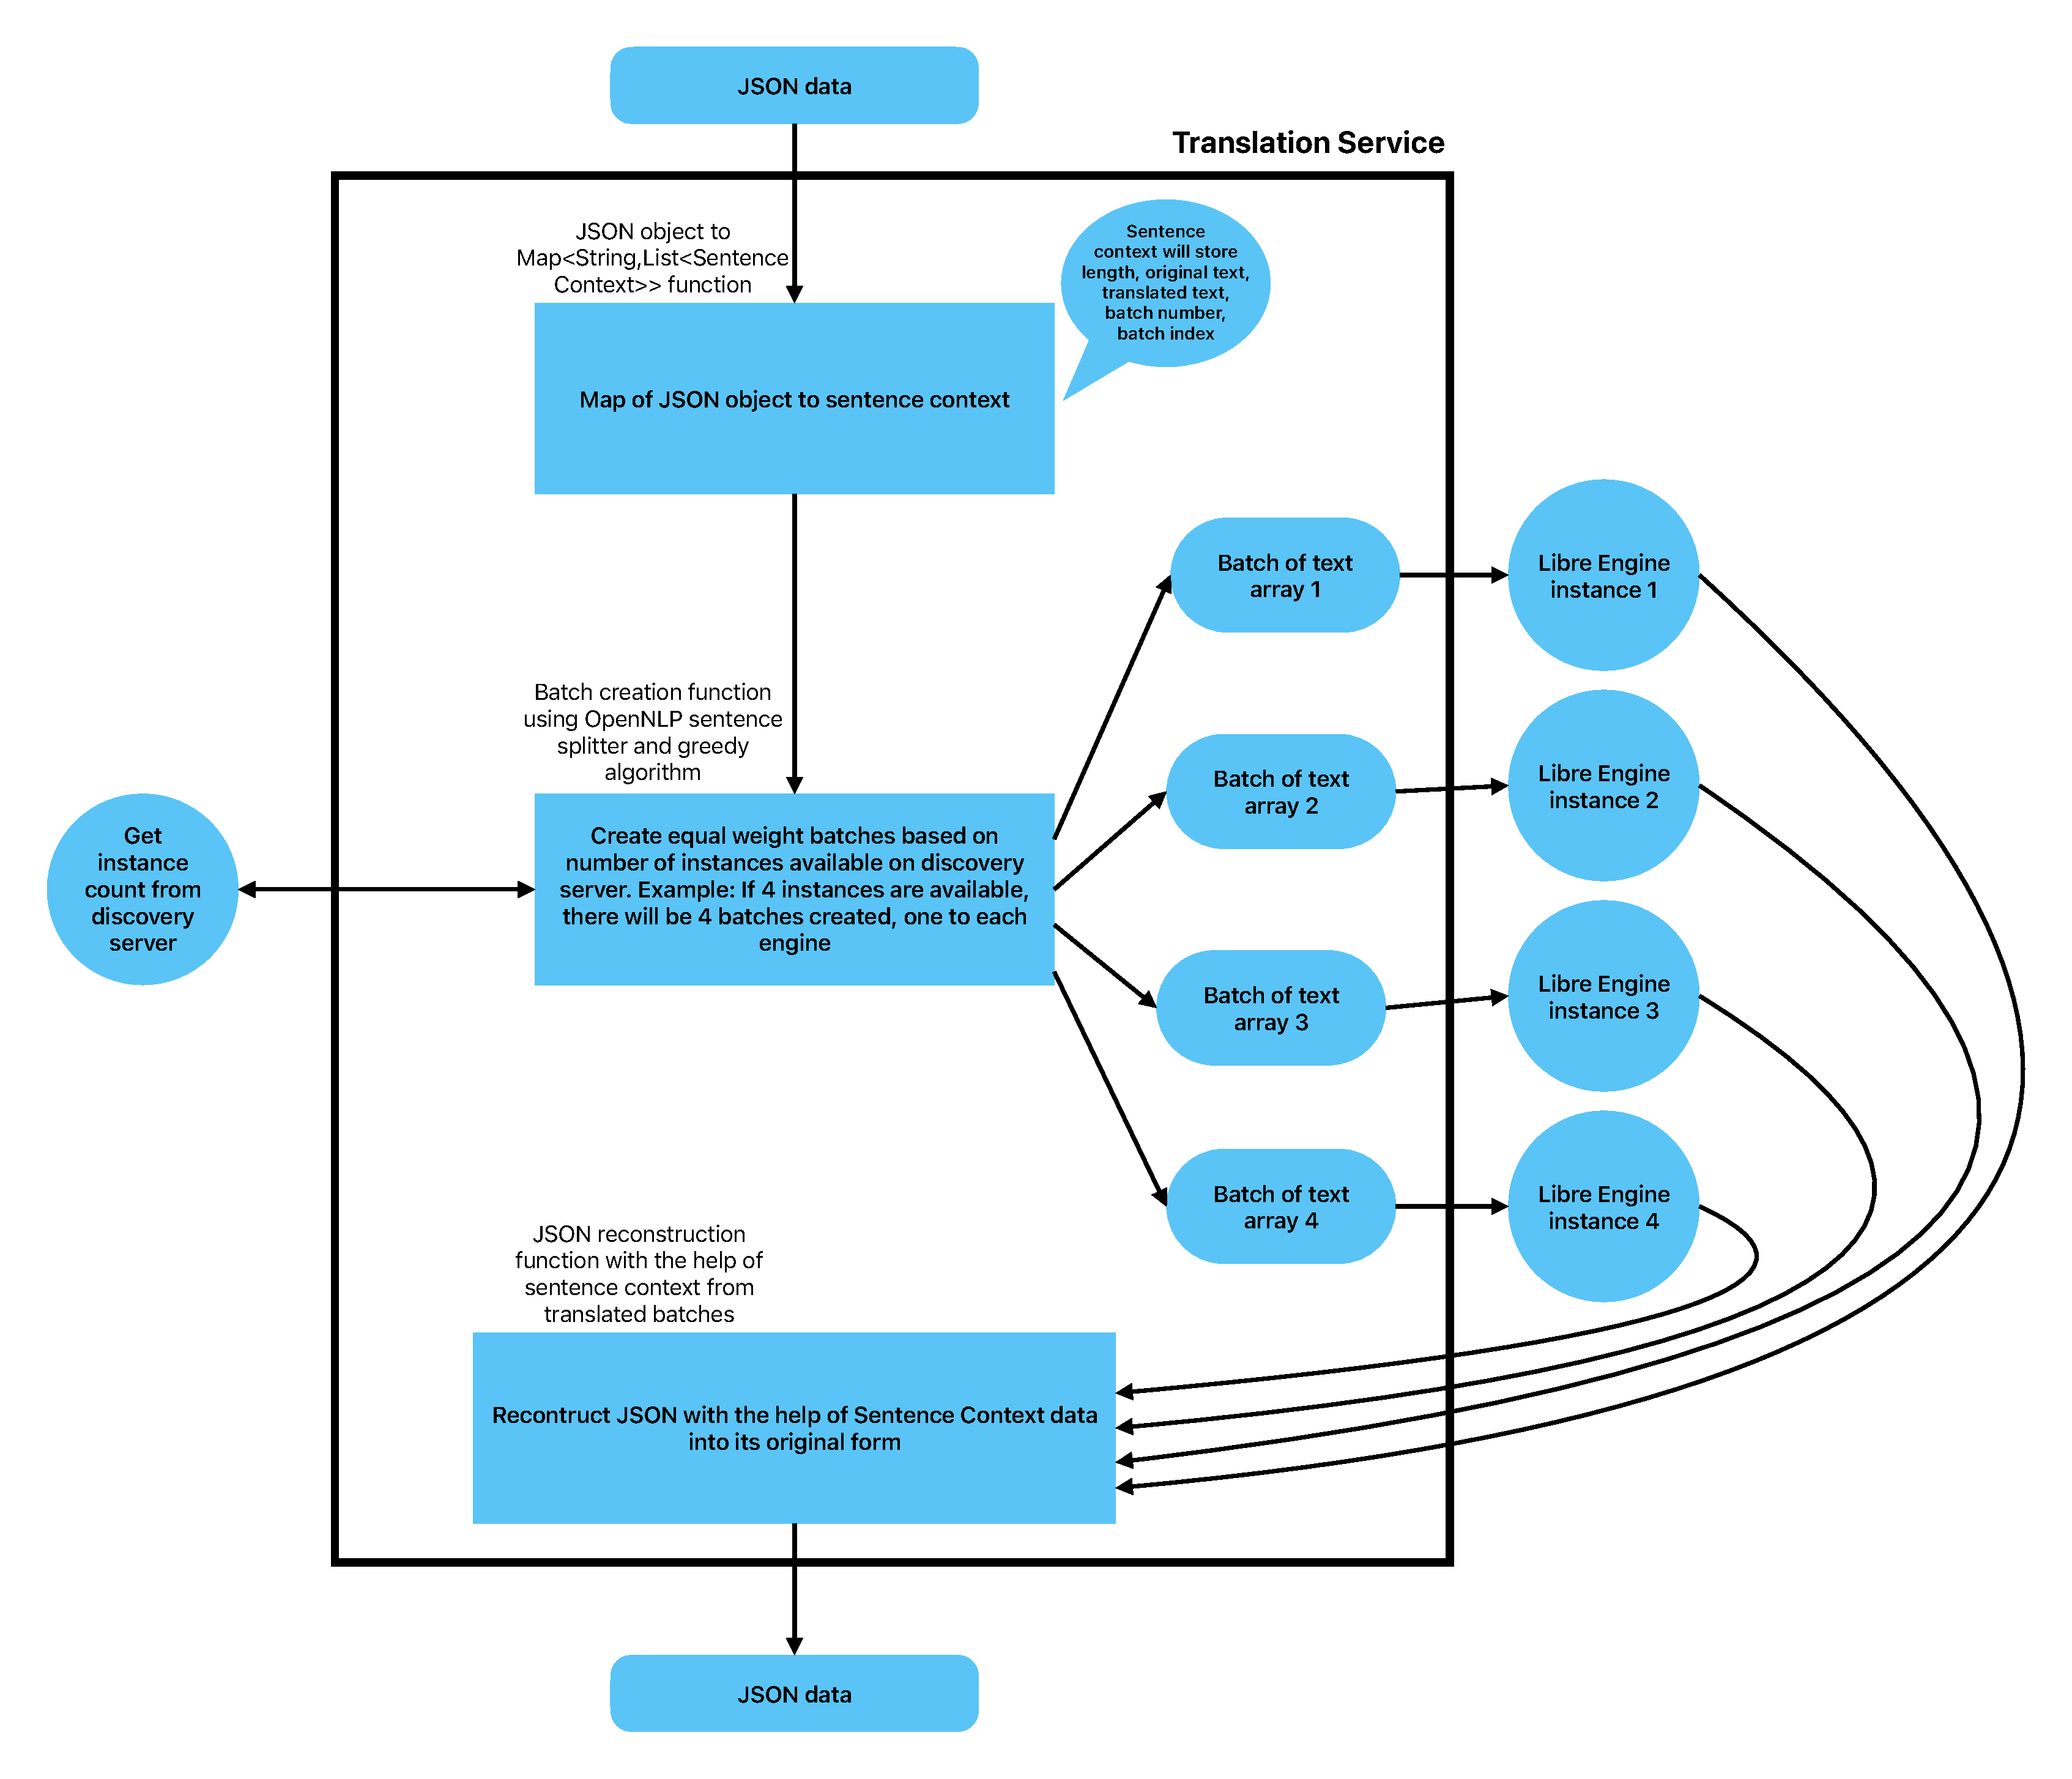
\includegraphics[width=1\linewidth]{images/Backend_Documents/Translation_Service.pdf}
    \caption{Translation request lifecycle}
    \label{fig:translation_engine_radar}
\end{figure}